\documentclass[final]{beamer}

\usepackage[size=custom,width=101.6,height=81.28,scale=1.15]{beamerposter} % Use the beamerposter package for laying out the poster
\usepackage{natbib} % Use the confposter theme supplied with this template
\usepackage{lmodern}
\usepackage{microtype}
\usepackage{amsmath}
\usepackage{amssymb}

\usetheme{confposter} % Use the confposter theme supplied with this template

\setbeamercolor{block title}{fg=ngreen,bg=white} % Colors of the block titles
\setbeamercolor{block body}{fg=black,bg=white} % Colors of the body of blocks
\setbeamercolor{block alerted title}{fg=white,bg=dblue!70} % Colors of the highlighted block titles
\setbeamercolor{block alerted body}{fg=black,bg=dblue!10} % Colors of the body of highlighted blocks
% Many more colors are available for use in beamerthemeconfposter.sty

%-----------------------------------------------------------
% Define the column widths and overall poster size
% To set effective sepwid, onecolwid and twocolwid values, first choose how many columns you want and how much separation you want between columns
% In this template, the separation width chosen is 0.024 of the paper width and a 4-column layout
% onecolwid should therefore be (1-(# of columns+1)*sepwid)/# of columns e.g. (1-(4+1)*0.024)/4 = 0.22
% Set twocolwid to be (2*onecolwid)+sepwid = 0.464
% Set threecolwid to be (3*onecolwid)+2*sepwid = 0.708

\newlength{\sepwid}
\newlength{\onecolwid}
\newlength{\twocolwid}
\setlength{\sepwid}{0\paperwidth} % Separation width (white space) between columns
\setlength{\onecolwid}{0.23\paperwidth} % Width of one column
\setlength{\twocolwid}{0.47\paperwidth} % Width of two columns
\setlength{\topmargin}{-0.5in} % Reduce the top margin size
%-----------------------------------------------------------

\usepackage{graphicx}  % Required for including images

\usepackage{booktabs} % Top and bottom rules for tables

%----------------------------------------------------------------------------------------
%   TITLE SECTION 
%----------------------------------------------------------------------------------------

\title{Dropout Object Detection and Neural Code Metric Learning}
\author{Philip Pham}
\institute{University of Washington}

%----------------------------------------------------------------------------------------

\begin{document}

\addtobeamertemplate{block end}{}{\vspace*{1ex}} % White space under blocks
\addtobeamertemplate{block alerted end}{}{\vspace*{1ex}} % White space under highlighted (alert) blocks

\setlength\belowdisplayshortskip{2ex} % White space under equations

\begin{frame}[t] % The whole poster is enclosed in one beamer frame

\begin{columns}[t] % The whole poster consists of three major columns, the second of which is split into two columns twice - the [t] option aligns each column's content to the top

\begin{column}{\onecolwid} % The first column

%----------------------------------------------------------------------------------------
%   OBJECTIVES
%----------------------------------------------------------------------------------------

  \begin{alertblock}{Objectives}

    This project consisted of several tasks with Common Objects in Context (COCO) dataset \citep{coco}.

    \begin{itemize}
    \item \textbf{Object detection:} Given an image, extract patches that contain an
      object and classify the object.
    \item \textbf{Metric learning:} Define a distance metric that compares patches such
      that patches of the same categories are close together, and patches of
      different categories are far apart.
    \end{itemize}
  \end{alertblock}

%----------------------------------------------------------------------------------------
%   INTRODUCTION
%----------------------------------------------------------------------------------------

\begin{block}{Introduction}
  The COCO dataset consists of 330,000 images. Each image is annotated with
  bounding boxes which contain objects belonging to one of 80 categories. Using
  this dataset, I explored several techniques covered in CSE 547 including
  neural networks, non-convex optimization, metric learning, and nearest
  neighbor methods.

  In particular, I explored different neural network architecures with various
  learning strategies before settling on a multi-layer perceptron model with
  dropout. For the metric learning, I attemped to use neural codes
  \citep{neural_codes}. Then, the nearest neighbor search is done using a ball
  tree.
\end{block}

\begin{block}{Methods and Materials}
  For object detection, regions were proposed with selective search
  \citep{selective_search}. Features for each image were given based on
  \cite{fast_rnn}. A fixed length feature vector was extracted for each patch
  using pooling \citep{pooling}.

  Using annotations provided by the COCO API, training, validation, and test
  datasets were constructed from the patches from the region proposoals with
  intersection over union (IoU) over 0.5 with a bouding box from an
  annotation. That patch was then labeled with the categories from the annotated
  bounding box. The training set consisted of 375,453 patches from 10,000
  images. The test set was 74,276 patches from 2,000 images, and the validation
  set was 75,620 patches from 2,000 images. Each patch had 11,776 features. From
  here, the problem can be seen as a multi-label classification problem. Models
  were trained with PyTorch \citep{pytorch}.

  The neural codes for the metric learning were extracted from the last hidden
  layer of the multi-layer perceptron used for object detection. To find nearest
  neighbors, a ball tree from \texttt{sklearn} was used \citep{scikit-learn}.
\end{block}

%------------------------------------------------

% \begin{figure}
% \includegraphics[width=0.8\linewidth]{placeholder.jpg}
% \caption{Figure caption}
% \end{figure}

%----------------------------------------------------------------------------------------

\end{column} % End of the first column

\begin{column}{\twocolwid} % Begin a column which is two columns wide (column 2)

\begin{columns}[t,totalwidth=\twocolwid] % Split up the two columns wide column

\begin{column}{\onecolwid}\vspace{-.6in} % The first column within column 2 (column 2.1)

%----------------------------------------------------------------------------------------
%   MATERIALS
%----------------------------------------------------------------------------------------

\begin{block}{Object Detection Models}

  Three types of models were trained for object detection. You can see the
  results in Table \ref{tab:model_comparison}. $L2$-regularization parameters
  and the number of hidden units were tuned to produce the smallest loss on the
  validation dataset. The idea behind using an MLP is that it enables
  weight-sharing in the hidden units. One might imagine certain animals or
  vehicles have common features that the model could learn together.

  \begin{table}
    \centering
    \begin{tabular}{lrr}
\toprule
Model &  Average Precision Score &      Loss \\
\midrule
Linear   &                 0.1750 &  0.1946 \\
  2-layer MLP &                 0.2198 &  0.1824 \\
  MLP with Dropout & 0.2351 & 0.1807 \\
\bottomrule
\end{tabular}

    \caption{Metrics are computed against the validation dataset.}
    \label{tab:model_comparison}    
  \end{table}

  The multi-layer perceptron with dropout performed best. It consisted of two
  hidden layers with 1,024 and 256 units, respectively. At each layer, dropout
  with $p = 0.5$ and ReLu activation functions were used. Dropout is a form of
  regularization that randomly zeroes outs a hidden unit during training
  \citep{dropout}.
\end{block}



% ----------------------------------------------------------------------------------------
\end{column} % End of column 2.1

\begin{column}{\onecolwid}\vspace{-.6in} % The second column within column 2 (column 2.2)

%----------------------------------------------------------------------------------------
%   METHODS
%----------------------------------------------------------------------------------------

\begin{block}{Model Evaluation}

  The mean average precision was
  0.254112 taken as
  unweighted average over the classes.

  If one looks at the class breakdown in Table
  \ref{tab:average_precision_score_by_class}, one sees that have
  under-represented classes have lower scores.
  \begin{table}
    \centering
    \scriptsize{\begin{tabular}{lrrr}
\toprule
      Label &  Training Observations &  Test Observations &  Average Precision Score \\
\midrule
    bicycle &                   9950 &               1847 &                 0.027483 \\
        car &                  56694 &              11010 &                 0.362490 \\
 motorcycle &                  13163 &               2757 &                 0.040598 \\
   airplane &                  15830 &               2529 &                 0.077730 \\
        bus &                  16103 &               2985 &                 0.087326 \\
      train &                   4568 &                873 &                 0.040963 \\
      truck &                  29670 &               6045 &                 0.117114 \\
       boat &                  15037 &               3179 &                 0.057605 \\
       bird &                  28911 &               6232 &                 0.314083 \\
        cat &                  12070 &               2778 &                 0.500823 \\
        dog &                  15957 &               2629 &                 0.240831 \\
      horse &                  22997 &               4966 &                 0.272576 \\
      sheep &                  34010 &               6046 &                 0.421672 \\
        cow &                  34359 &               7271 &                 0.318933 \\
   elephant &                  23508 &               3972 &                 0.454776 \\
       bear &                   3827 &                578 &                 0.018140 \\
      zebra &                  25923 &               5720 &                 0.578105 \\
    giraffe &                  19805 &               4243 &                 0.642767 \\
\bottomrule
\end{tabular}
}
    \caption{Class breakdown of average precision score.}
    \label{tab:average_precision_score_by_class}
  \end{table}
  
\end{block}

%----------------------------------------------------------------------------------------

\end{column} % End of column 2.2

\end{columns} % End of the split of column 2 - any content after this will now take up 2 columns width

%----------------------------------------------------------------------------------------
%   IMPORTANT RESULT
%----------------------------------------------------------------------------------------

\begin{alertblock}{Results}

  The best unweighted mean average precision on the test set was
  0.254112. With the
  learned metric, the nearest neighbor was of the same category 24\% of the
  time.
\end{alertblock} 

% ----------------------------------------------------------------------------------------

\begin{columns}[t,totalwidth=\twocolwid] % Split up the two columns wide column again

  \begin{column}{\onecolwid} % The first column within column 2 (column 2.1)
    
    \begin{block}{Model Training}

      \begin{figure}
        \centering
        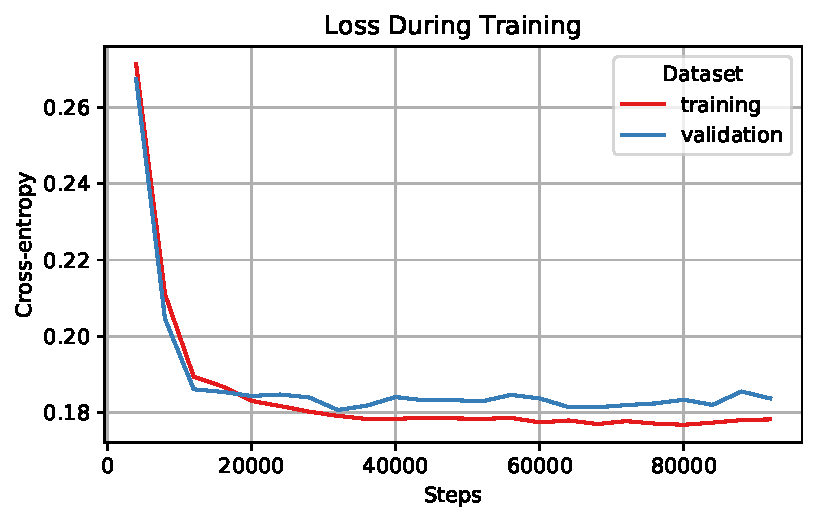
\includegraphics[scale=1.5]{../project/object_detection/training_loss.pdf}
        \caption{Loss and the mean average precision score (not shown) were
          calculated after every 4,000 steps}
        \label{fig:training_loss}
      \end{figure}

      The multi-layer perceptron with dropout was trained with stochastic
      gradient descent with Nesterov's momentum with a learning rate of 0.03 and
      momentum parameter of 0.9 \citep{momentum}. The batch size was 128, and
      the L2-regularization parameter was $\lambda = 0.0025$. The model was
      trained for 32 epochs but it can seen in Figure to have converged much
      earlier in Figure \ref{fig:training_loss}.
\end{block}

%----------------------------------------------------------------------------------------

\end{column} % End of column 2.1

\begin{column}{\onecolwid} % The second column within column 2 (column 2.2)

\begin{block}{Metric Learning}

  \cite{neural_codes} and \cite{imagenet} suggest that the top layer of a
  network may summarize an image, so I thought to try extract that layer to use
  as an embedding. Let $f$ be my neural network. We can write $f = g \circ h$,
  where $h$ takes the patch features and outputs 256-dimensional vector that
  forms the last hidden layer. Then, the distance metric for two patches $P$ and
  $P^\prime$ is
  $d\left(P,P^\prime\right) = \left\lVert h\left(P\right) -
    h\left(P^\prime\right)\right\rVert_2$. Results can be found in Figure
  \ref{fig:metric_average_precision_score} and Table
  \ref{tab:metric_learning_class}. The nearest neighbor is of the same category
  about a quarter of time. In some rare instances, like \texttt{bird},
  \texttt{cat}, \texttt{dog}, and \texttt{cow}, the next few neighbors are more
  likely to be of the same category.
  
  \begin{figure}
    \centering
    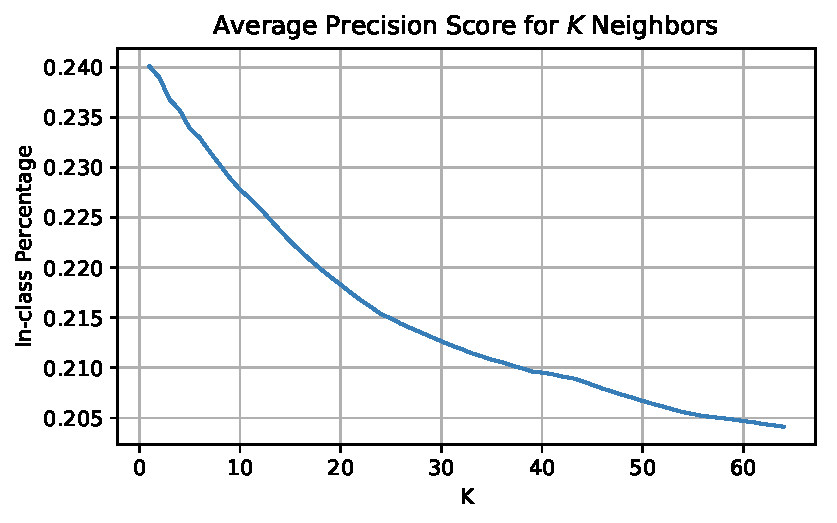
\includegraphics[scale=1.5]{../project/metric_learning/metric_average_precision_score.pdf}
    \caption{For $K$ up to 64, the average precision score was calculated.}
    \label{fig:metric_average_precision_score}
  \end{figure}
  
\end{block}

\end{column} % End of column 2.2

\end{columns} % End of the split of column 2

\end{column} % End of the second column

\begin{column}{\onecolwid} % The third column


  \textrm{\scriptsize{\begin{table}
    \centering
    \begin{tabular}{lrrrrr}
\toprule
            & \multicolumn{5}{l}{Number of Neighbors} \\
      Label &               K = 1 &     K = 3 &     K = 5 &    K = 10 &    K = 15 \\
\midrule
    bicycle &            0.042793 &  0.046547 &  0.044257 &  0.043187 &  0.043919 \\
        car &            0.314220 &  0.309779 &  0.307115 &  0.291930 &  0.287312 \\
 motorcycle &            0.051215 &  0.049844 &  0.049047 &  0.046280 &  0.045134 \\
   airplane &            0.061684 &  0.063662 &  0.062554 &  0.058600 &  0.058521 \\
        bus &            0.106321 &  0.100110 &  0.094995 &  0.095543 &  0.091804 \\
      train &            0.044499 &  0.040379 &  0.037824 &  0.034981 &  0.037165 \\
      truck &            0.147673 &  0.134968 &  0.126489 &  0.121318 &  0.120335 \\
       boat &            0.098957 &  0.088207 &  0.083908 &  0.075624 &  0.075603 \\
       bird &            0.208440 &  0.216303 &  0.214121 &  0.208521 &  0.197925 \\
        cat &            0.287394 &  0.301850 &  0.301360 &  0.302536 &  0.289599 \\
        dog &            0.289124 &  0.296166 &  0.284507 &  0.271753 &  0.266249 \\
      horse &            0.242839 &  0.223252 &  0.217355 &  0.206529 &  0.198905 \\
      sheep &            0.296334 &  0.295381 &  0.294618 &  0.289876 &  0.291456 \\
        cow &            0.285961 &  0.286681 &  0.288553 &  0.289590 &  0.279952 \\
   elephant &            0.256494 &  0.251366 &  0.255687 &  0.261892 &  0.267474 \\
       bear &            0.127273 &  0.101818 &  0.097455 &  0.082364 &  0.073576 \\
      zebra &            0.379962 &  0.376348 &  0.370869 &  0.351582 &  0.333310 \\
    giraffe &            0.350071 &  0.340798 &  0.336445 &  0.339981 &  0.335691 \\
\bottomrule
\end{tabular}

    \caption{For each patch, the percentage of neighbors belonging to the
      same one was calculated and then averaged.}
    \label{tab:metric_learning_class}
  \end{table}}}

%----------------------------------------------------------------------------------------
%   CONCLUSION
%----------------------------------------------------------------------------------------

\begin{block}{Conclusion}

  My model does not perform nearly as well as other models in the
  literature. For example, \cite{benchmark} achieve a baseline mean average
  precision score of 0.415.

  Some possible improvements include getting more computing power and using more
  the dataset and exploring more complicated network architecures like
  convolutions and residual networks.

  One promising way to improve my approach to metric learning that builds on my
  current approach would be to adopt a \emph{siamese architecture}
  \citep{siamese}.

\end{block}

%----------------------------------------------------------------------------------------
%   ADDITIONAL INFORMATION
%----------------------------------------------------------------------------------------

\begin{description}
\item[Code:] \href{https://gitlab.cs.washington.edu/pmp10/cse547}{https://gitlab.cs.washington.edu/pmp10/cse547}  
\end{description}

%----------------------------------------------------------------------------------------
%   REFERENCES
%----------------------------------------------------------------------------------------

\begin{block}{References}

{\scriptsize \bibliographystyle{chicago}
\bibliography{../project/references}}

\end{block}

\end{column} % End of the third column

\end{columns} % End of all the columns in the poster

\end{frame} % End of the enclosing frame

\end{document}
